\chapter{Preliminary Experiments}
\label{chapter:chapter04}

Before the overall comparison of algorithms took place, it was necessary to test the methodology defined in Chapter~\ref{chapter:chapter03}, each component of the solution model was tested individually, to make sure that the experiments in Chapter~\ref{chapter:chapter04} ran correctly and the check if the optimisation made sense.\\

For these experiments, there were three different steps taken. First, some of the objective functions were tested one by one to see if they achieve our requirements. Then, there is a description of how synthetic data-set was created. Finally, some initial experiments regarding the comparison between algorithms took place, as a first approach to test the objective functions and operators, as well as the data-set defined.

\section{Experiments regarding objective functions}

Some of the objective functions used for the research had a very straightforward approach. The standard $\sigma$ deviation represents how much variety of different levels of experience there is within a group. For function $Gs$, subtraction is the representation of the distance to the ideal group size.

To define the objective functions for interests similarity and the participation style it was necessary to perform additional experiments. Since this can be accomplished in different ways and it was not known which was the most adequate. These experiments are described in the following subsections. \\

\subsection{Interests distance function}

For these experiments, four different students were randomly generated with their respective interest set $I_i$, as it was described in Section~\ref{subsection:interests_similarity}. The purpose is to find the distance between $I_1$ and $I_2$. Ideally, we want to have a metric that is a continuous value between zero and one, so it does not need normalisation. Several similarity metrics found in \cite{SeyedShirkhorshidi2015AData} and \cite{Sung-HyukChaComprehensiveFunctions} were tested discarding the ones that did not evaluate to a value from zero to one. This is because when there are no common interests between the students, in some of the metrics it leads to a division by zero. In the end, two metrics were selected for comparison, the cosine distance (CD) and Pearson correlation coefficient (PC).\\

The results of this experiment can be seen in Figure~\ref{table:results_interests_comp}. Here several comparisons of each pair of students are observed, using both CD and PC. With the difference between both, for comparison. This was done using the sets of interests specified in Table~\ref{table:sample_interests}, % in the same way it was specified in Chapter~\ref{chapter:chapter03}, 
where each interest is given a normalised distance to each other.\\

\begin{table}[]
\centering
\begin{tabular}{lcccc}
\hline
Interests & $S_1$      & $S_2$      & $S_3$      & $S_4$      \\ \hline
Business       & 0.50 & 0.00 & 0.00 & 0.00       \\
Property       & 1.00 & 0.00 & 0.00 & 0.00       \\
Entertainment  & 0.33 & 0.00 & 0.00 & 0.50       \\
Games          & 0.50 & 0.00 & 0.00 & 0.00       \\
Gambling       & 1.00 & 0.00 & 0.00 & 0.00       \\
Films          & 0.50 & 0.00 & 0.00 & 1.00       \\
Animated Films & 1.00 & 0.00 & 0.00 & 0.00       \\
Family         & 0.00 & 0.50 & 0.00 & 0.25       \\
Dating         & 0.00 & 1.00 & 0.00 & 0.00       \\
Marriage       & 0.00 & 0.00 & 0.00 & 1.00       \\
Fitness        & 0.00 & 0.50 & 0.00 & 0.00       \\
Running        & 0.00 & 1.00 & 0.00 & 0.00       \\
Pets           & 0.00 & 0.50 & 0.00 & 1.00       \\
Hobbies        & 0.00 & 0.33 & 0.33 & 0.50       \\
Dogs           & 0.00 & 1.00 & 0.00 & 0.00       \\
Travel         & 0.00 & 0.00 & 0.50 & 0.00       \\
Beaches        & 0.00 & 0.00 & 1.00 & 0.00       \\
Arts           & 0.00 & 0.00 & 0.50 & 0.00       \\
Guitar         & 0.00 & 0.00 & 1.00 & 0.00       \\
Dance          & 0.00 & 0.00 & 1.00 & 0.00       \\ \hline
    \end{tabular}
    \caption{Sample interests by student.}
    \label{table:sample_interests}
\end{table}

\begin{table}[!htb]
    \begin{subtable}{.5\linewidth}
        \centering
        
            \begin{tabular}{ll}
            \hline
            Metric            & Value  \\
            \hline
            Cosine Similarity &  0.00  \\
            Pearson + 1       &  0.56  \\
            Pearson           & -0.43  \\
            CD - Pearson      &  0.43  \\
            \hline
            \end{tabular}\\
            \\
            \caption{Comparison between $S_1$ and $S_2$.}\\ 
            \\
            
            \begin{tabular}{ll}
            \\
            \hline
            Metric            & Value  \\
            \hline
            Cosine Similarity &  0.00  \\
            Pearson + 1       &  0.60  \\
            Pearson           & -0.39  \\
            CD - Pearson      &  0.39  \\
            \hline
            \end{tabular}\\
            \\
            \caption{Comparison between $S_1$ and $S_3$.}\\
            \\
            
            \begin{tabular}{ll}
            \\
            \hline
            Metric            & Value  \\
            \hline
            Cosine Similarity &  0.18  \\
            Pearson + 1       &  0.86  \\
            Pearson           & -0.13  \\
            CD - Pearson      &  0.31  \\
            \hline
            \end{tabular}\\
            \\
            \caption{Comparison between $S_1$ and $S_4$.}\\
            \\
            
    \end{subtable}
    \begin{subtable}{.5\linewidth}
      \centering
      
            \begin{tabular}{ll}
            \hline
            Metric            & Value  \\
            \hline
            Cosine Similarity &  0.029 \\
            Pearson + 1       &  0.65  \\
            Pearson           & -0.34  \\
            CD - Pearson      &  0.37  \\
            \hline
            \end{tabular}\\
            \\
            \caption{Comparison between $S_2$ and $S_3$.}\\
            \\
            
            \begin{tabular}{ll}
            \\
            \hline
            Metric            & Value  \\
            \hline
            Cosine Similarity &  0.21  \\
            Pearson + 1       &  0.91  \\
            Pearson           & -0.08  \\
            CD - Pearson      &  0.30  \\
            \hline
            \end{tabular}\\
            \\
            \caption{Comparison between $S_2$ and $S_4$.}\\
            \\
            
            \begin{tabular}{ll}
            \\
            \hline
            Metric            & Value  \\
            \hline
            Cosine Similarity &  0.04  \\
            Pearson + 1       &  0.71  \\
            Pearson           & -0.28  \\
            CD - Pearson      &  0.32  \\
            \hline
            \end{tabular}\\
            \\
            \caption{Comparison between $S_3$ and $S_4$.}\\
            \\
            
    \end{subtable} 
    \caption{Comparison between the sample students.}
    \label{table:results_interests_comp}
\end{table}

\subsection{Participation style Function}

The participation style function aims to reduce the \textit{quantity of silence} in the conversations of a group to a minimum. Therefore, the objective function should have a relationship between this \textit{quantity of silence}. In the literature, there is no already a metric or a mathematical function that is able to tell how much silence will be produced in a determined conversation. What it has been found is a model created by Benne and Sheats~\cite{FunctionalRoles} that assigns a \textit{Functional Role} label to the intention each of the utterances has in a conversation. It is assumed that there must be a correlation between the \textit{quantity of silences} in a conversation and the \textit{Functional Role} or a combination of \textit{Functional Roles} in a conversation.\\

To understand the behaviour in a conversation, it was proposed to make brief data analysis of a group of conversation and check the interaction between the silence quantity and the functional roles. For this analysis, it was found a well-known data-set AMI meeting corpus~\cite{mccowan2005ami}, which has previously been used in other studies~\cite{dong2012modeling, Matsuyama2015Four-participantParticipant}. The data-set includes several conversations of different meetings with different people, with markers of time indicating when each utterance occur, along with with some notes and an accompanying video. Some of the meetings found in this data-set had also been labelled with their correspondent \textit{Functional Role} for each utterance by~\cite{dong2012modeling}.\\

The meetings used for these analysis have the following names: "ES2002d", "ES2008b", "ES2008d", "ES2009d" and "IS1003d". The first task was to analyse the \textit{quantity of silences} and their duration. Fortunately, each utterance also has a start time and an end time, so the proportion of the conversation which was silence is considered as the time in which no utterance is occurring.\\

For each meeting, the total silence time in seconds was considered as the proportion corresponding to the total conversation time. The results can be seen in Table~\ref{table:ami_times}. Here, it can be observed the number of silences in seconds and the total time each conversation was in silence proportionally. It can be observed, for example, that the meeting IS1003d had less silence time in comparison to ES2008d.\\

\begin{table}[H]
    \centering
    \begin{tabular}{ccc}
        \hline    
        & Total Silence time & Silence proportion \\ \hline
        ES2002d & $6861.49s$         & $72.89\%$  \\
        ES2008b & $7867.38s$         & $75.24\%$  \\
        ES2008d & $6973.49s$         & $78.23\%$  \\
        ES2009d & $5963.49s$         & $70.49\%$  \\
        IS1003d & $5514.33s$         & $66.78\%$  \\
        \hline
    \end{tabular}
    \caption{Quantity of silences and their proportion by meeting.}
    \label{table:ami_times}
\end{table}

One of the conversation functional roles of Benne and Sheats is described as ''protagonism´´. This infers that a person making an utterance with this intention is starting to talk about a specific topic, not just responding by the utterance made by others. It was inferred that this specific role may have some correlation with the lack of silences. The next step involved measuring the \textit{protagonistic proportion} and \textit{protagonistic time} of each of the participants in the conversation. This is for all the utterance they made, how many were \textit{protagonistic} and for all the time they spoke, how much of it was \textit{protagonistic} respectively.\\

Tables~\ref{table:res_ES2008d}~and~\ref{table:res_IS1003d} show the \textit{protagonistic proportion} and \textit{protagonistic time} for each participant in the conversation with the most (ES2008d) and the less (IS1003d) \textit{quantity of silences} respectively. As it can be seen in Table~\ref{table:res_ES2008d}, the meeting ES2008d has only brief protagonisms by a single person in the conversation, while in Table~\ref{table:res_IS1003d}, the meeting IS1003d has a homogeneous amount of \textit{protagonisms} by all of their participants.\\

\begin{table}[H]
    \centering
    \begin{tabular}{ccc}
    \hline
    Participant & Protagonism proportion & Protagonistic time \\ \hline
    A           & $9.46\%$                & $3.97\%$            \\
    B           & $0.58\%$                & $0.23\%$            \\
    C           & $4.19\%$                & $1.86\%$            \\
    D           & $15.9\%$                & $5.16\%$
             \\
    \hline
    \end{tabular}
    \caption{Protagonism proportion for the Meeting IS1003d.}
    \label{table:res_IS1003d}
\end{table}

\begin{table}[H]
    \centering
    \begin{tabular}{ccc}
    \hline
    Participant & Protagonism proportion & Protagonistic time\\ \hline 
    A           & $9.29\%$               & $3.2\%$            \\
    B           & $0.0\%$                & $0.0\%$            \\
    C           & $0.0\%$                & $0.0\%$            \\
    D           & $0.0\%$                & $0.0\%$            \\
    \hline
    \end{tabular}
    \caption{Protagonism proportion for the Meeting ES2008d.}
    \label{table:res_ES2008d}
\end{table}

Finally, the number of participations was compared to the average participation and the summation of these participations, shown in Table~\ref{table:results_ami}. Here we proposed an inverse correlation to the sum of participations $\frac{1}{\sigma}$ as the metric for improving the number of participations and therefore lowering the \textit{quantity of silence}, as it can be seen in Table~\ref{table:results_ami}, a low value of it represents a positive impact on the number of participations.\\

\begin{table}[H]
    \centering
    \begin{tabular}{ccccc}
    \hline
    Conversation & Participations proportion & Average  of paticipation & $\Sigma$ & $\frac{1}{\Sigma}$ \\ \hline
    ES2008b      & $24.75\%$                 & $0.80\%$                                                              & $23.17\%$  & $4.3$               \\
    ES2008d      & $24.16\%$                 & $5.79\%$                                                              & $3.21\%$   & $31.17$              \\
    ES2002d      & $27.11\%$                 & $4.29\%$                                                              & $17.15\%$  & $5.83$               \\
    ES2009d      & $29.51\%$                 & $2.43\%$                                                                & $9.72\%$   & $10.29$              \\
    IS1003d      & $33.21\%$                 & $2.81\%$                                                                & $11.23\%$  & $8.90$              \\
    \hline
    \end{tabular}
    \caption{Results of the conversation analysis.}
    \label{table:results_ami}
\end{table}

It should be noted that this, by no means, is considered a strong data analysis, nor the objective function should be considered as definitive. But, as a first approach, and considering the information that could be gathered at the moment, it serves its purpose for the sake of this research.\\

\section{Synthetic data-set creation}
\label{section:synthetic_dataset}

To calculate the value for each objective function described in Section~\ref{section:objective_functions}, it is necessary to consider some features about each student regarding their experience level, their interests and their participation style.\\

The experience level is represented as a numerical quantity. For the interests, it was considered a fixed size of three interests for each one of the students, and a feature representing the participation style was considered as the percentage of the Benne and Sheats role~\cite{FunctionalRoles} of "Protagonist" that a student has on average in a conversation.\\

Since these features have never been used in any other scenario together, there was not a specific data-set that included all of them. Therefore, the data-set was created in such a way that it resembles what a real data-set would look like once data is gathered for each of the features. To this end, the mean and standard deviation were used to determine the statistical distributions. In the following subsections is discussed how data was obtained and other important details for the data-set creation.\\

In the following subsection is described where the metrics (mean and standard deviation) comes from and why were they used.\\

\subsection{Experience Level} 

While there is no distribution information for the language levels for CEFR specifically, the IELTS has data about the frequency distributions by percentage~\cite{ielts_demographic_data_2018} which has a distribution by a given level. Fortunately, these levels have their equivalence in the CEFR scale, as can be observed in Table~\ref{table:results_levels}.\\

\begin{table}[H]
    \centering
    \begin{tabular}{cc}
    \hline
    CEFR Level & Proportion \\
    \hline
    A0         & 0.33\%     \\
    A1         & 0.33\%     \\
    A2         & 0.33\%     \\
    B1         & 13.0\%     \\
    B2         & 48.0\%     \\
    C1         & 36.0\%     \\
    C2         & 2.0\%      \\
    \hline
    \end{tabular}
    \caption{The distribution by each level.}
    \label{table:results_levels}
\end{table}

\subsection{Interests} 

The social network Facebook has a database of interests separated by population and regions. This data corresponds to the ontology presented in Section~\ref{section:facebook_ad_platform} and Section~\ref{subsection:interests_similarity}. The main purpose of the Facebook Ad platform~\cite{facebook_business} is to build marketing campaigns.\\

When a user of this platform consults the potential marketing segment, filtered by specific interest, a number known as \textit{potential reach} is shown. This number was acquired for each of the interests in the ontology to figure out the proportion of the population for each interest.\\

The ontology contains overall categories (such as "Business and Industry" or "Hobbies"), this, however, was not considered for the distribution estimation, because they represented very general interests. Therefore, only interests from the third level onwards in the ontology were considered. Part of the distributions of interests can be seen in Table~\ref{table:results_interests}. \\

\begin{table}[H]
    \centering
    \begin{tabular}{lc}
    \hline
    Interest name              & Proportion \\
    \hline
    Television programme       & 62.94\%    \\
    Restaurants                & 45.88\%    \\
    Vehicles                   & 27.25\%    \\
    Sports                     & 13.00\%    \\
    Music                      & 8.21\%     \\
    Arts and music             & 5.29\%     \\
    Travel                     & 5.11\%     \\
    Films                      & 4.61\%     \\
    Reading                    & 4.51\%     \\
    Consumer electronics       & 4.43\%     \\
    Games                      & 4.18\%     \\
    Shopping                   & 3.68\%     \\
    Beauty                     & 3.49\%     \\
    Live events                & 3.21\%     \\
    Politics and social issues & 2.96\%     \\
    Food                       & 2.87\%     \\
    Computers                  & 2.48\%     \\
    Pets                       & 2.29\%     \\
    Clothing                   & 2.07\%     \\
    Drinks                     & 2.04\%     \\
    \hline
    \end{tabular}
    \caption{The first 20 Interests and their proportion.}
    \label{table:results_interests}
\end{table}

\subsection{Participation style}

For the participation style, the same data-set as for defining the function was used, the AMI meeting corpus. Since we established the metric to be used as the \textif{proportion of protagonisms}, the mean and standard deviation were calculated directly per person in each conversation. The results of this can be seen in Table~\ref{table:participation_results}. Here, the mean and standard deviation of the \textif{proportion of protagonisms} for each of the participants in each of the conversations is shown.\\

\begin{table}[H]
    \centering
    \begin{tabular}{ll}
    \hline
    Protagonism mean               & $9.67\%$ \\
    Protagonism standard deviation & $6.66\%$ \\
    \hline
    \end{tabular}
    \caption{Results for the Participation Analysis.}
    \label{table:participation_results}
\end{table}

\section{Exploratory Experiments}

Before comparing the proposed algorithms, several exploratory experiments took place to understand how the objective functions and the proposed operators behave. This also serves as the first comparison of a simple meta-heuristic, a population-based meta-heuristic, and a multi-objective algorithm. All algorithms were subject to similar parameters, described as follows.\\

\begin{itemize}
    \item A data-set of {10,001} was used. The mutation operator described in 
    Section~\ref{section:mutation_operator} at a $1/n$ rate.

    \item For the single objective algorithms, the same weight for all the functions was considered.
    
    \item For the population-based algorithms GA and NSGA-II the crossover operator defined in Section~\ref{section:crossover_operator} was used at a $0.9$ rate.

    \item Also, for the population-based algorithms, a population of $p=40$ was considered. 
    
    \item All the algorithms ran for over $10,000$ evaluations, which means $10,000$ steps for LS, and $250$ generations for GA and NSGA-II
\end{itemize}

\subsection{Single-Objective Optimisation}

For the SOA, a Weighted Sum was used, shown in Equation~\ref{weighted_function}, considering each of the objective functions previously defined. This also serves as the basis for comparison between these single objective and multi-objective experiments.\\

\begin{itemize}
\item Function for the group size \(f_{1}\)
\item Function for the interests similarity \(f_{2}\)
\item Function for the similarity of experience level \(f_{3}\)
\item Function for the participation style \(f_{4}\)
\end{itemize}

\begin{equation} \label{weighted_function}
    f_{agg} = \sum_{i=1}^4 \omega_i f_i
\end{equation}

\subsubsection{Local Search}

For the first experiment, a LS algorithm was used, due to is one of the most simple meta-heuristics for single-objective optimisation according to the literature \cite{boussaid2013survey}. As it can be seen in Figure~\ref{fig:local_search}, from a random solution the algorithm manages to improve until it gets stuck in a local minimum.\\

\begin{figure}
    \centering
    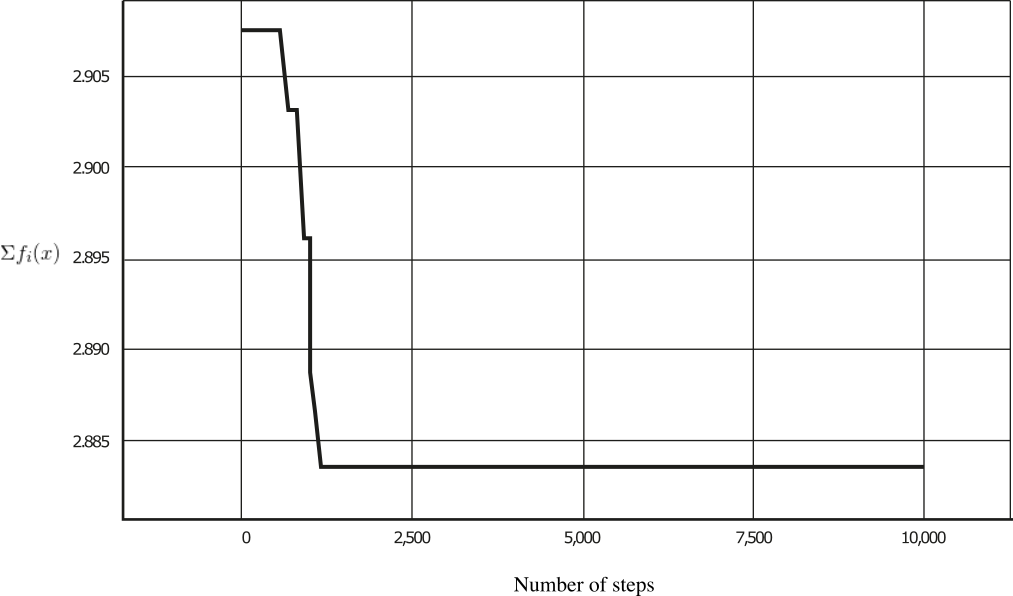
\includegraphics[width=\textwidth]{images/local_search.png}
    \caption{Performance of the LS algorithm.}
    \label{fig:local_search}
\end{figure}

\subsubsection{Genetic Algorithm}

LS is a meta-heuristic that only makes a single change per step. However, it was also necessary to test the proposed crossover operator in a population-based approach. An experiment using a GA was also tested with similar parameters to LS, with the number of iterations corresponding to the number of generations. As can be seen in Figure~\ref{fig:genetico}, the algorithm manages to improve for the first $100$ steps until it reaches a local minimum, then it continues moving to worse solutions.

\begin{figure}
    \centering
    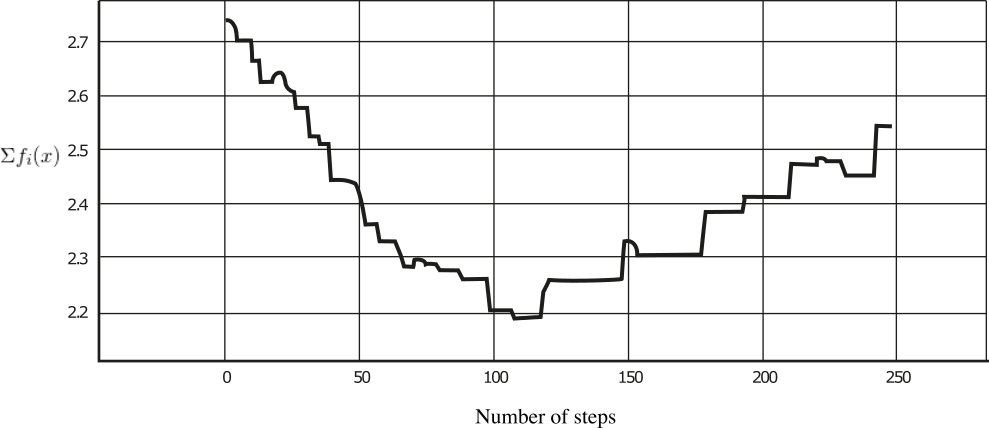
\includegraphics[width=\textwidth]{images/genetic_algorithm.png}
    \caption{Performance of the single objective GA.}
    \label{fig:genetico}
\end{figure}

\subsection{Multi-Objective Algorithm}

For the single-objective optimisation, it was decided to use NSGA-II, since is one of the most common algorithms found in the literature and has mostly the same parameters as the single objective genetic algorithm.\\

To compare it to the single-objective algorithms, $f_{agg}$ was evaluated for each of the solutions in the obtained front in each step. The graph in Figure~\ref{fig:multiobjetivo} is made from the best solutions from the fronts produced in each step considering $f_{agg}$.\\

As can be seen in Figure~\ref{fig:multiobjetivo} the algorithm is stuck at several local minima, but it manages to continue improving. It also should be noticed that it improves significantly better than its single-objective counterparts.

\begin{figure}
    \centering
    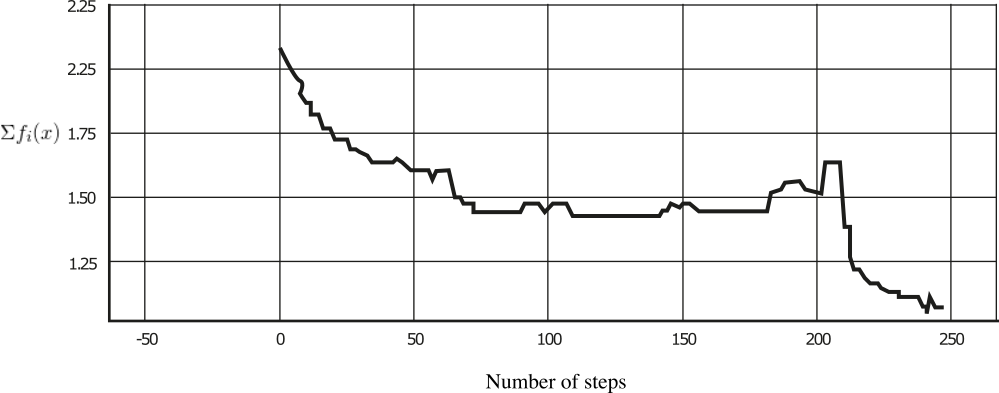
\includegraphics[width=\textwidth]{images/multiobjective.png}
    \caption{Performance of the NSGA-II.}
    \label{fig:multiobjetivo}
\end{figure}

\section{Preliminary conclusions}

After analysing the results, it can be noticed that there is very little variation with the aggregated function $f_{agg}$, this is mostly because for this experimentation phase the same weights were considered for all the functions. However considering that not all functions have the same minimum and maximum values, there was a clear need to normalise them. This is done in the experiments in Chapter~\ref{chapter:chapter05}. It should also be noticed that for the LS algorithm $f_{agg}$ seems to become trapped in the local minima, further evidence of this is GA and NSGA-II being able to find a better solution. Finally, NSGA-II had the best performance overall, which may be a clue that MOA may be able to outperform SOA. It should also be noticed that despite using a large data-set of {10,001} students for these experiments, the local minima appear after $100$ steps.